\chapter{Generating Unit Tests from a UML Activity}
\label{chap:testgeneration}
In this chapter we will present an algorithm that generates unit tests for C functions from their \textbf{U}nified \textbf{M}odeling \textbf{L}anguage\textsuperscript{\texttrademark} (UML) activity model. The test generation process is divided in five steps. %Each steps of the presented algorithm performs a model there is a comprehensive interface defined. 
Each step can be seen as model--to--model, model--to--text, or text--to--model transformation with the input and output language or model specified. The architecture makes it particularly easy to replace any of the five steps or extend it with additional features. We do not only specify an algorithm for generating unit tests from a UML model but also a framework for building further algorithms that generate unit tests from arbitrary input models. If, for instance, another input language specifying a control flow graph will be used then only the first step would need a few changes. In some steps we will even specify alternative transformations.\\
Our approach for automated generation of test data is based on mathematical programming and the approach for finding relevant control flow paths is based on a breadth first search with early infeasible path recognition.
\section{General Overview of the Workflow} %BAM DIGGER DIE EINLEITUNG IST GUT!!!
\label{sec:testgenerationOverview}
\begin{figure}
\includegraphics[width=\textheight,height=\textwidth,angle=270]{pics/workflow.pdf}
\label{fig:workflowOverview}
\caption{Overview of the workflow for unit test generation}
\end{figure}
The transformation from an UML activity diagram to a C++ unit test code is divided in five steps. Those five steps are: \nameref{sec:Normalisation}, \nameref{sec:atcg2Ampl}, \nameref{sec:pathsearch}, \nameref{sec:testgenerationSolving}, and finally \nameref{sec:testgenerationUnitTestSynthesis}. Here we want to give a brief overview of those five steps. Each of these steps as well as the interfaces between them will be described in detail in the following sections.\\
In the first step, \nameref{sec:Normalisation}, we check some design rules, parse all embedded OCL constraints, and map the relevant parts from the UML model onto a simplified meta model of an activity. Throughout the next step we generate a mathematical program out of our simplified test model. We use the AMPL language for specifying a rigorous mathematical program. The third step, \nameref{sec:pathsearch}, is a path search where we can find all control flow paths, or those that are necessary to fulfil some coverage criterion of choice. We call a control flow path from an initial node to a final node of an activity \emph{abstract test case}. In the fourth step, \nameref{sec:testgenerationSolving}, we have each abstract test case encoded as input data for the AMPL model generated during the second step. The AMPL model will be solved by a state--of--the--art solver that interfaces with AMPL. For each abstract test case the solver was able to find valid test data we will store the data in a \emph{test case model}. This test case model serves as input for the last step. During \nameref{sec:testgenerationUnitTestSynthesis}, we take the generated solution of the mathematical program and put the values in place within compilable and executable C++ unit test code. An overview of the complete workflow of our approach is given in Figure \ref{fig:workflowOverview}. There we see an activity diagram showing the five steps of our algorithm and within each step the sub--tasks are visible. Each of the depicted central buffer nodes will hold the output of one step of the algorithm. The labelled input pins at the actions indicate which task accesses which previously generated item.\\
We want to outline two special features of our algorithm. Early infeasible path recognition as described in Section \ref{sec:EarlyInfeasiblePathRecognition} enables us to recognise sub--paths for which no valid input data exists during the path search in the third step. When early infeasible path recognition is used the third and fourth step are interfering with each other. In this case test data is already generated in the \nameref{sec:pathsearch}. %When infeasible paths need to be detected already during the search of control flow paths the third and fourth step are directly interfering with each other. How we can determine infeasible sub--paths and bound the search for abstract test cases will be explained in the . 
Another feature of the specified algorithm is that it generates boundary values for each abstract test case. For each control flow path in an activity there is a set of input values that will satisfy all constraints along this path and thus presents suitable test data for this abstract test case. In testing, bugs often are likely to be triggered when a point at the edge of this set is selected as test data. How we are assuring that a boundary value will be found during test data generation will be explained in Section \ref{sec:boundaryValueSelection}.
%1. Normalise Model, 2.Make model mathematical Rigorous, 3. Search for Control flow Paths. 4 Solve Mathematical Program for the found Control flow Paths to generate specific Input and output Data. 5. Generate Unit Tests
\section{Normalisation}
\label{sec:Normalisation}
The \textbf{U}nified \textbf{M}odeling \textbf{L}anguage\textsuperscript{\texttrademark} (UML) specifies about 250 modelling elements each having several references and attributes. An algorithm interpreting every element that is defined in the UML becomes overly complex. We interpret only a subset of the UML consisting of 16 different modelling elements. For a complete reference of the UML elements we refer to the UML2.3  superstructure specification \cite{UML23Superstructure}. In industrial applications a model will usually contain the complete specification for a product consisting of thousands of objects and containing elements we are not interested in. Through the references of any object within a model we can navigate to any other object within the model. In order to not get lost in such a model when generating unit tests from it, we need to slice out the relevant sub--model and perform a pre--processing step to ensure our algorithm does not run into error conditions. Especially the contained OCL expressions need to be parsed and checked for conformity with the subset of OCL our algorithm is able to handle correctly. The input of the \nameref{sec:Normalisation} step is an UML \UMLType{Activity} from which we traverse all relevant attributes and references and store each bit of information needed in consequent steps in our own unambiguous intermediate representation. The input model can be discarded after this step. All consequent steps we will exclusively use our own intermediate representation and no more access the original UML model. Throughout this section and the rest of this thesis we will print specific modelling elements and associations of the UML in a special font, for example \UMLType{Activity} and \UMLReference{ownedNodes}, to make it clear that the UML modelling element or the UML association as described in the UML specification \cite{UML23Superstructure} is meant. 
\subsection{Design Rules for the Test Model} %Structural Design rules
\subsubsection{Structural Design Rules}
\begin{figure}
\begin{center}
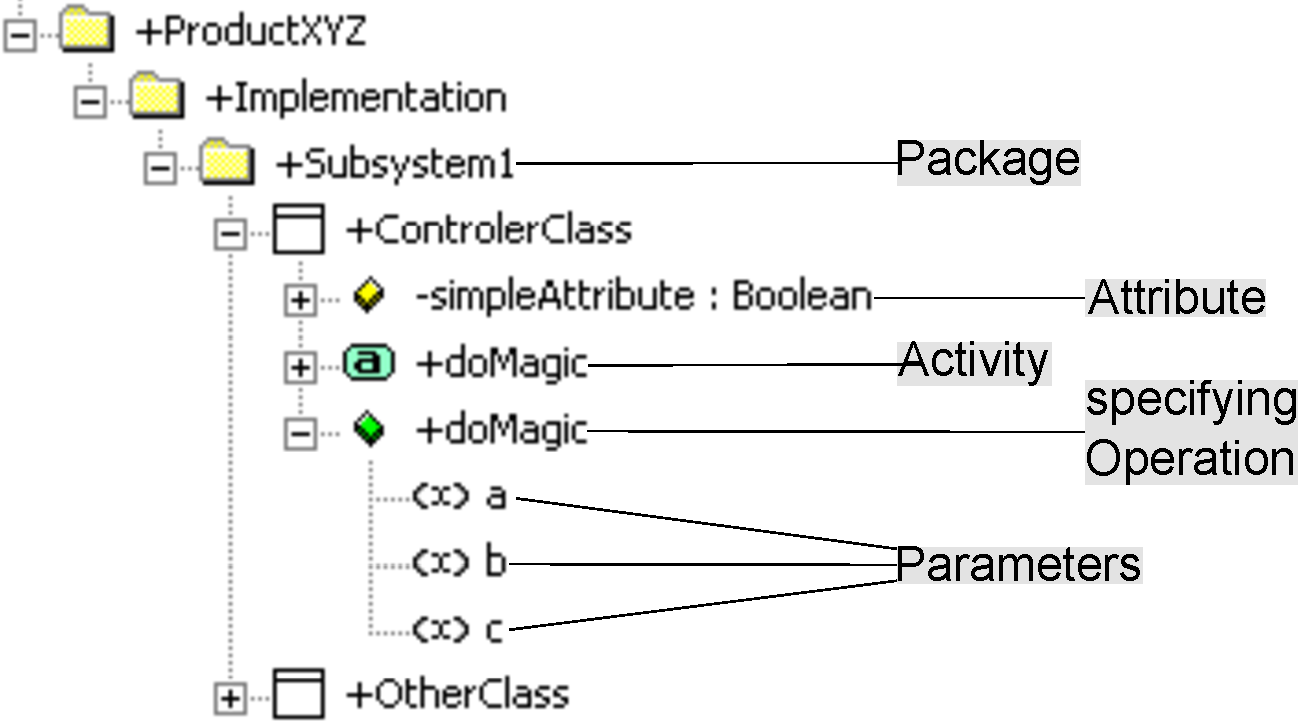
\includegraphics[width=0.5\textwidth]{./pics/ModelTreeView2.pdf}
\end{center}
\caption{Example of a valid structured model}
\label{fig:StructureExample}
\end{figure}
For our test generation we assume the models to comply to certain design rules. The input \UMLType{Activity} is an \UMLReference{ownedActivity} of a \UMLType{Class}. The \UMLType{Class} containing the \UMLType{Activity} itself is contained by a \UMLType{Package}. There is an \UMLType{Operation} specifying the \UMLType{Activity}. This specifying \UMLType{Operation} is either a sibling in the UML tree structure and has the same name as the \UMLType{Activity} or is explicitly specified by the \UMLReference{specification} reference of the \UMLType{Activity}. The specifying \UMLType{Operation} will be needed when parsing OCL constraints in Section \ref{sec:OCLParsing}. In Figure \ref{fig:StructureExample} we see a tree view of an UML model where those requirements are met.
\subsubsection{OCL design rules}
\label{sec:OCLDesignRules}
Further we assume that the embedded textual OCL constraints are either contained within a \UMLType{LiteralString} element or an \UMLType{OpaqueExpression} with the according \UMLReference{language} value set to `OCL'. We support a strict subset of the OCL language. The Extended Backus--Naur Form (EBNF) of the supported OCL subset is shown in Algorithm \ref{alg:OCLEBNF}. Any parsed OCL expression must be an instance of the <Bool> production rule.
\begin{algorithm}
\begin{description}
\item[<Bool> ::=] <LogicalOperation> | <RelationOperation> | <BooleanLiteral> | <BooleanVariable> ;
\item[<LogicalOperation> ::=] <Bool>, <LogicalOpSymbol>, <Bool> ;
\item[<LogicalOpSymbol> ::=] "and" | "or" ;
\item[<RelationOperation> ::=] <Number>, <RelationOpSymbol>, <Number> ;
\item[<RelationOpSymbol> ::=] "<" | ">" | "<=" | ">=" | "=" | "<>" ;
\item[<Number> ::=] <ArithmeticOperation> | <IntegerLiteral> | <RealLiteral> | <IntVariable> | <RealVariable> ;
\item[<ArithmeticOperation> ::=] <Number>, <ArithmeticOpSymbol>, <Number> ;
\item[<ArithmeticOpSymbol> ::=] "+" | "-" | "*" | "/" ;
\item[<BooleanLiteral> ::=] "true" | "false" ;
\item[<IntegerLiteral> ::=] [ "-" | "+" ], <Digit>, \{<Digit>\} ;
\item[<RealLiteral> ::=] [ "-" | "+" ], <Digit>, \{<Digit>\}, ".", \{<Digit>\} ;
\item[<Digit> ::=] "0" | "1" | "2" | "3" | "4" | "5" | "6" | "7" | "8" | "9" ;
\item[<BooleanVariable> ::=] ?OCL expression evaluating to a \UMLType{Property} or \UMLType{Parameter} of type boolean? ;
\item[<IntegerVariable> ::=] ?OCL expression evaluating to a \UMLType{Property} or \UMLType{Parameter} of type integer? ;
\item[<RealVariable> ::=] ?OCL expression evaluating to a \UMLType{Property} or \UMLType{Parameter} of type real? ;
\end{description}
\caption{Extended Backus--Naur Form of supported OCL subset}
\label{alg:OCLEBNF}
\end{algorithm}
\subsection{A Meta Model Suitable for Automated Unit Test Generation}
\label{sec:TestCaseGraph}
The developed unit test generation algorithm does not work directly on an UML model but on an \emph{activity test case graph}. The activity test case graph contains only those details from the UML meta model that are really necessary for the unit test generation. Since it contains only parsed OCL expressions as abstract syntax trees it is much more suitable for the transformation into a mathematical program.\\
The activity test case graph is defined as an extension of a more general \emph{abstract test case graph} model. The abstract test case graph meta model was tailored to fit activity diagrams as well as UML state machine diagrams in order to be able to apply algorithms not only to activity diagrams but also to state machine diagrams. This common abstract meta model is also a provision to be able to reuse existing test case generation algorithms from ParTeG \cite{ParTeG} for \UMLType{Activities}. The Eclipse plug--in developed along with this thesis will be integrated with ParTeG. ParTeG is a test generator for activity diagrams with advanced support for different coverage criteria.
% XXX no reference to ParTeG before
% 
%????
%Figure \ref{fig:ATCGMetamodel} shows the complete meta model of the activity test case graph including all components from the abstract test case graph.
%\begin{figure}
%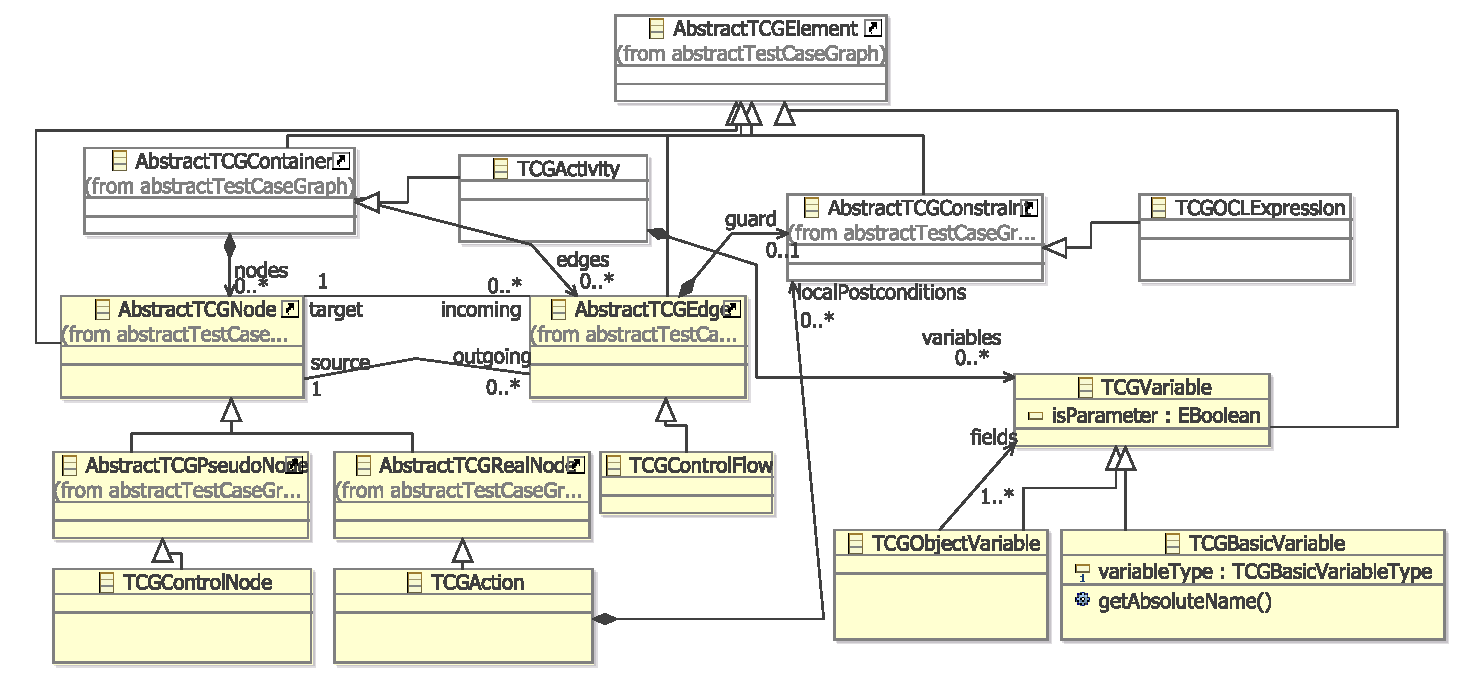
\includegraphics[width=\textwidth]{./pics/ATCGMetamodel.pdf}
%\label{fig:ATCGMetamodel} 
%\caption{Complete meta model of activity test case graph}
%\end{figure}
%????
\subsubsection{Abstract Test Case Graph}
\begin{figure}
\begin{center}
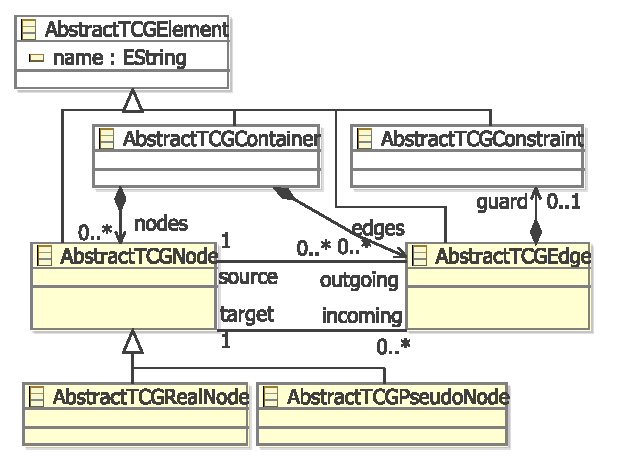
\includegraphics[width=0.8\textwidth]{./pics/AbstractTestCaseGraph.pdf}
\end{center}
\caption{Meta model of the abstract test case graph}
\label{fig:AbstractTCGMetaModel}
\end{figure}
An abstract test case graph is a directed graph consisting of nodes (AbstractTCGNode) and edges (AbstractTCGEdge). Each edge has a source and a target node. Each node can have multiple outgoing and multiple incoming edges.
A node can be either a pseudo node (AbstractTCGPseudoNode) or a real node (AbstractTCGRealNode). A pseudo node is a node that can be inserted in the middle of an edge without changing the semantics of the test model. Edges can have a guard condition of type AbstractTCGConstraint. Such a graph is contained by a container (AbstractTCGContainer). The container has a singular reference to one of its nodes exposing this as the initial node. The class diagram of the abstract test case graph meta model is shown in Figure \ref{fig:AbstractTCGMetaModel}.\\
The semantic of the activity test case graph is like a Petri net. When executing an abstract test case graph we have at the beginning a token in the initial node that can move along the enabled edges. An edge is enabled when its guard condition is true. We say that a node is being executed when a token resides in the node.
\subsubsection{Activity Test Case Graph}
\begin{figure}
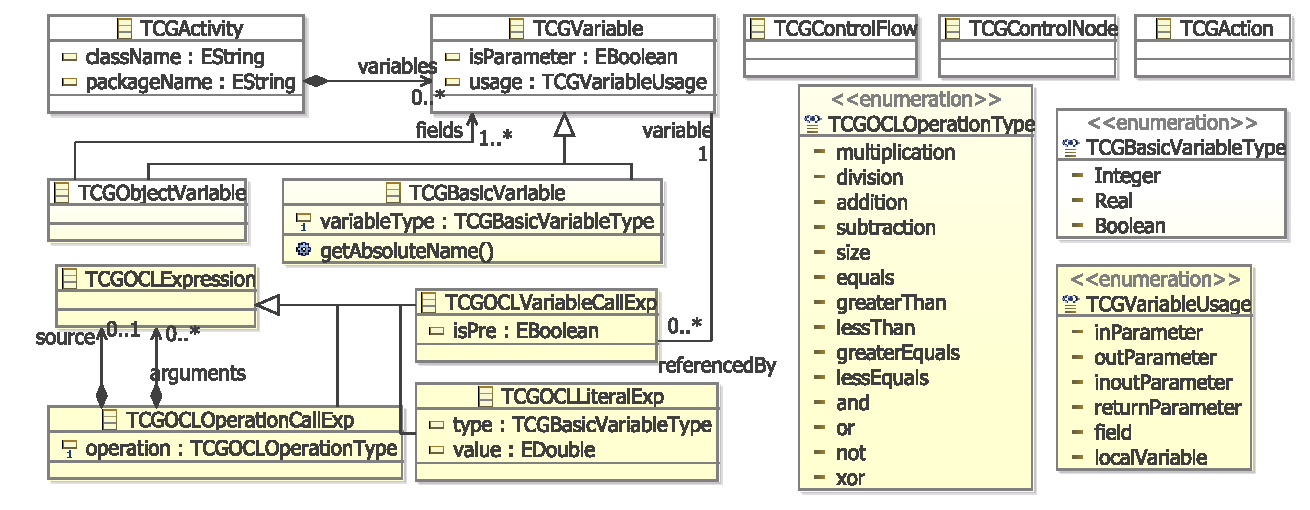
\includegraphics[width=\textwidth]{./pics/ActivityTestCaseGraph.pdf}
\caption{Meta model of the activity test case graph}
\label{fig:ActivityTCGMetaModel}
\end{figure}
An activity test case graph is an extension to the abstract test case graph especially tailored for test generation from \UMLType{Activities}. The activity test case graph models control flow and constraints on variables. The constraints are required to hold at different points during execution of the activity test case graph. Its meta model is shown in Figure \ref{fig:ActivityTCGMetaModel}.\\
The TCGActivity is an extension of the AbstractTCGContainer. TCGAction, TCGControl-Node, and TCGControlFlow refine the types AbstractTCGRealNode, AbstractTCGPseudo-Node, and AbstractTCGEdge respectively. The main extensions to the abstract test case graph meta model are the variables (TCGVariable), the elements of an abstract syntax tree (TCGOCLExpression) to express constraints, and the TCGAction.
\paragraph{TCGAction} A TCGAction can, in addition to its super--type, contain arbitrary many localPostconditions of the type AbstractTCGConstraint. A local post--condition has the semantics that it has to be true after the execution of the action. This implies potentially changing some variables throughout the execution of the action.
\paragraph{TCGOCLExpression}
TCGOCLExpression is a subtype of AbstractTCGConstraint. A TCGOCLExpression can either be a TCGOCLOperation call with a source and arguments, or a TCGOCLLiteralExpression holding a literal value and its data type, or a TCGOCLVariableCallExp referencing a TCGVariable. The isPre attribute of TCGOCL-VariableCallExp denotes whether the original OCL expression contained an \verb=@pre= token. TCGOCLExpression and its subtypes form a simplified OCL abstract syntax tree.
\paragraph{TCGVariable}
A TCGVariable can be one of two subtypes: either a TCGBasicVariable or a TCGObjectVariable. An object variable is put together by one or more other variables. A basic variable has a variableType attribute holding a TCGBasicVariableType literal. The TCGBasicVariableType literal represents one of the types that our algorithm can handle: integer, real, and boolean. A TCGVariable is a placeholder for a value. When the isParameter attribute is true it can only hold one value throughout the execution of the TCGActivity, otherwise it can change its value during each execution of a TCGAction.
\subsection{Transforming an UML Activity Diagram to an Activity Test Case Graph}
\label{sec:uml2atcg}
\begin{figure}
\begin{center}
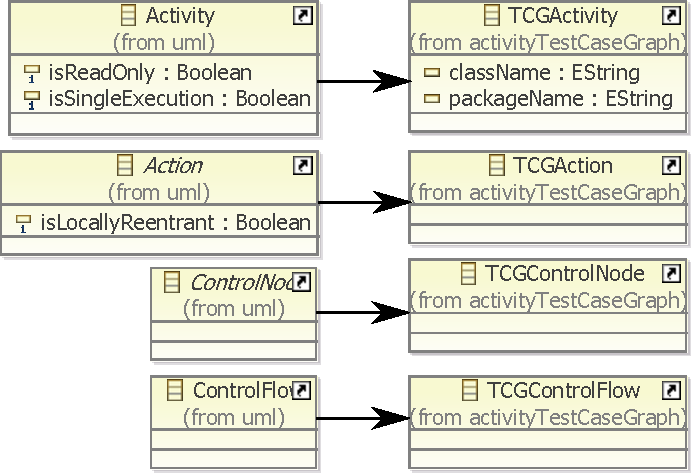
\includegraphics[width=\textwidth]{./pics/UML2TCGTransformation.pdf}
\end{center}
\caption{Straightforward mapping from UML elements to activity test case graph elements}
\label{fig:UML2TCGTranformation}
\end{figure}
An instance of the activity test case graph meta model serves as a normalised input model. We use a model--to--model transformation to transform an \UMLType{Activity} from a UML model into an activity test case graph. In many cases the transformation is straightforward: for one element in the UML model the corresponding element in the activity test case graph is produced. When one element of the UML model is mapped to one element of the activity test case graph model we call the UML element \emph{source element} and the created element in the activity test case graph model \emph{target element}. The straight forward mappings from one source element to one target element are shown in Figure \ref{fig:UML2TCGTranformation}.
\subsubsection{Mapping UML Elements to Activity Test Case Graph Elements}
\paragraph{Activity}
A UML \UMLType{Activity} is transformed into a TCGActivity. For the C++ unit test synthesis described in Section \ref{sec:testgenerationUnitTestSynthesis} the name of the containing \UMLType{Class} of the source element as well as the full pathname to the \UMLType{Package} containing this \UMLType{Class} need to be stored. The class name and the full pathname will be stored in the property fields of the TCGActivity. For each \UMLType{Activity} all of its \UMLReference{ownedNodes} as well as \UMLReference{ownedEdges} are considered for transformation.
\paragraph{Action} \UMLReference{OwnedNodes} of an \UMLType{Activity} that are a subtype of \UMLType{Action} are transformed into a TCGAction. The \UMLType{Action}s \UMLReference{localPostcondition}s may contain textual OCL that will be parsed. The detailed semantics of special subtypes of an \UMLType{Action} is neglected.
\paragraph{ControlNode} \UMLReference{OwnedNodes} of the \UMLType{Activity} that are a subtype of \UMLType{ControlNode} are transformed into TCGControlNodes. That means they are pseudo nodes. It is assumed that there is only one UML \UMLType{InitialNode} whose target element is referenced by the TCGActivity as initial node.
\paragraph{ControlFlow} Based on the \UMLReference{ownedEdges} association of the \UMLType{Activity} we find \UMLType{ControlFlow}s that are transformed into TCGControlFlows. If there is a \UMLType{ValueSpecification} contained in the \UMLReference{guard}, the potentially contained textual OCL needs to be parsed.
\subsubsection{Parsing OCL Constraints}
\UMLType{Constraint}s can be found in the \UMLReference{localPostcondition} reference of an \UMLType{Action}. Each \UMLType{Constraint} holds a \UMLType{ValueSpecification} in its \UMLReference{specification} reference. A \UMLType{ControlFlow} can hold a \UMLType{ValueSpecification} in its \UMLReference{guard} reference.\\
\UMLType{Constraint}, \UMLType{ValueSpecification}, and \UMLType{Property} as well as \UMLType{Parameter} can not be transformed straightforwardly. The transformation will be done in three steps. First, textual OCL expressions will be extracted from \UMLType{ValueSpecification}s and then the textual OCL expression will be parsed. When the OCL expression was parsed correctly the parser returns an abstract syntax tree of this expression. In the third step the elements of this abstract syntax tree will be transformed to TCGOCLExpressions and all \UMLType{Properties} and \UMLType{Parameters} referenced by the OCL abstract syntax tree will be transformed into TCGVariables.\\
We ensure that only those OCL expressions are in the activity test case graph that later on can be transformed into an AMPL model as explained in in Section \ref{sec:atcg2Ampl}. There might for example be \UMLReference{ownedAttribute}s of a \UMLType{Class} that are not changed by any of the transformed \UMLType{Actions} and whose value do not have any influence on any of the transformed \UMLType{ControlFlow}'s \UMLReference{guard}. The activity test case graph will not contain any TCGVariable representing such an irrelevant \UMLType{Property} or \UMLType{Parameter}.
\paragraph{Extracting Textual OCL}
\UMLType{LiteralString} and \UMLType{OpaqueExpression} are subtypes of \UMLType{ValueSpecification} potentially containing textual OCL expressions. For a \UMLType{LiteralString} we will try to parse its \UMLReference{value} as OCL. For an \UMLType{OpaqueExpression} we will first check whether the \UMLReference{language} attribute contains the value `OCL' and try to parse the corresponding value of the \UMLReference{body} attribute. If the \UMLReference{language} attribute does not contain the value `OCL' then we will try to parse the concatenation of all \UMLReference{body}s of the \UMLType{OpaqueExpression}.
\paragraph{Parsing Textual OCL}
\label{sec:OCLParsing}
For details of the \textbf{O}bject \textbf{C}onstraint \textbf{L}anguage (OCL) we refer to the OCL 2.3 specification \cite{OCL}. For this thesis we consider three types of constraints: \emph{invariants}, \emph{post--conditions} and \emph{guard conditions}. Every OCL constraint is parsed with respect to a \emph{context}. The context specifies the evaluation of the \verb=self= keyword and which other variables and parameters are accessible from the OCL expression.\\
Textual OCL found inside a \UMLType{Constraint} contained by the \UMLReference{ownedRule} reference of either the \UMLType{Activity}, or its containing \UMLType{Class} will be interpreted as invariant. Invariants need to be true before the \UMLType{Activity} is executed and after the execution of the \UMLType{Activity} has finished. The OCL expressions found within \UMLReference{guards} of \UMLType{ControlFlows} are required to evaluate to true, whenever the \UMLType{ControlFlow} is traversed. We are parsing the invariants as well as guards according to the OCL specification as invariants of the specifying \UMLType{Operation}. \\
\UMLType{Actions} can contain multiple \UMLType{Constraints} within their \UMLReference{localPostcondition} reference. Every post--conditions is required to hold after the execution of the \UMLType{Action} containing it. Only in post--conditions the OCL \verb=@pre= is allowed. With \verb=@pre= we refer to the value of a variable before the execution of the \UMLType{Action}. Any textual OCL found within a \UMLReference{localPostcondition} will be parsed as post--condition in the context of the specifying \UMLType{Operation}.
That means for every parsed OCL expression all attributes of the \UMLType{Class} as well as all \UMLReference{ownedParameters} of the specifying \UMLType{Operation}, and all properties of the containing \UMLType{Packages} are accessible, but only in local post--conditions the \verb=@pre= is valid.
\paragraph{Transforming the Abstract Syntax Tree}
%\begin{figure}
%\includegraphics[width=\textwidth]{}
%\end{figure}
If the OCL parser was supplied with a valid OCL expression for the context that was assumed then it will return an abstract syntax tree for the parsed OCL expression. We assume the parsed OCL complied with the rules explained in Section \ref{sec:OCLDesignRules} and the OCL abstract syntax tree returned consists of those tokens specified in Algorithm \ref{alg:OCLEBNF}.\\ %We explain the transformation of the of the abstract syntax tree in bottom up fashion starting with the terminals and then moving upwards.
% explain the rules for transforming an OCL abstract syntax tree  We are interested in a subset of the OCL abstract syntax trees namely the subset presented in Section \ref{sec:OCL}. 
<BooleanLiteral>, <IntegerLiteral>, and <RealLiteral> are transformed into a TCGOCLLiteralExp. Its value is stored in double precision floating point format. The type attribute of the target element is set according to the type of the source element. For the type boolean a value of $0.0$ means false and $1.0$ means a true.\\
<BooleanVariable>, <IntegerVariable>, and <RealVariable> tokens are transformed into TCGOCLVariableCallExp elements. If the original OCL token was tagged with an \verb=@pre= then the isPre attribute is set to true otherwise it is false. <BooleanVariable>, <IntegerVariable>, and <RealVariable> elements represent an arbitrary OCL expression that evaluates either to a \UMLType{Property} or a \UMLType{Parameter}. The \UMLType{Property} or \UMLType{Parameter} pointed to by the expression will be transformed into a TCGVariable and the variable reference of the TCGOCLVariableCallExp will be set to point to this TCGVariable.\\
We transform a <LogicalOpSymbol>, <RelationOpSymbol>, or <ArithmeticOpSymbol> into the enumeration literal of the TCGOCLOperationType enumeration that matches the token represented by the source element. The token \verb�=� matches for example the equals enumeration literal.\\
Each <LogicalOperation>, <ArithmeticOperation>, and <RelationalOperation> will be transformed into a TCGOCLOperationCallExp. The value of the operation attribute will be obtained by transforming the <RelationalOpSymbol>, <LogicalOpSymbol>, or <ArithmeticOpSymbol> contained in the source element. The target element of the first operand of each operation will be stored in the source reference of the TCGOCLOperation. The target element of the second operand will be stored in the arguments reference of the TCGOCLOperationCallExp.\\
The productions <Bool> and <Number> in Algorithm \ref{alg:OCLEBNF} are there to keep the EBNF notation more readable. No TCGOCLExpression element is generated for them but the transformation of a <Bool> or <Number> element will transform the contained abstract syntax tree node and return the result of this transformation.\\
Every root TCGOCLExpression directly contained by a TCGAction, TCGControlFlow, or TCGActivity gets its name property set. The transformation ensures that every root TCGOCLConstraint has a globally unique name. In the original UML model it is not the case that each \UMLType{Constraint} or \UMLType{ValueSpecification} has a globally unique name.
\paragraph{Transforming Properties and Parameters}
UML \UMLType{Properties} or \UMLType{Parameters} referenced by a <BooleanVariable>, <IntegerVariable>, or <RealVariable> element will be transformed into a TCGVariable. All TCGVariables are contained by the variables reference of the root element of the activity graph, the TCGActivity.\\
For \UMLType{Parameters} and \UMLType{Properties} we need to check their \UMLReference{type} reference. If the \UMLReference{name} of the \UMLType{Type} is one out of a list of names that can be mapped to a literal of the TCGBasicVariableType enumeration then a TCGBasicVariable is created for it and its variableType field set accordingly to the enumeration literal that is either integer, real, or boolean. The exact mapping of \UMLReference{names} of the \UMLType{Type} to a TCGvariableType is implementation specific. One could for example map from a \UMLType{Type} named `uint32{\_}t' to integer.\\
If a \UMLType{Parameter} was transformed into a TCGBasicVariable then the isParameter field is set to true, indicating that this variable has been a \UMLType{Parameter}. For \UMLType{Properties} the isParameter field of the target element will be set to false.\\
The field usage of the TCGBasicVariable can take values from the enumeration TCGVariableUsage. This information will be needed when creating the C or C++ unit tests as described in Section \ref{sec:testgenerationUnitTestSynthesis}. If the TCGBasicVariable was created to represent a \UMLType{Parameter} then its usage can be inParameter, outParameter, inoutParameter, or returnParameter. The value of the usage field for a transformed \UMLType{Parameter} is determined by the value of the \UMLReference{direction} field of the original \UMLType{Parameter}. If the source element of a TCGBasicVariable was a \UMLType{Property} then its usage is field.
%according to the OCL specification as explained in Section \ref{sec:OCL}. 
% When the textual expression was successfully parsed according to the OCL specification we hold an abstract syntax tree of the OCL Expression as explained in \ref{sec:OCL}. The elements from the OCL abstract syntax tree are then transformed into TCGOCLExpressions. Whenever a 
%transform then only those \UMLType{Properties} and \UMLType{Parameters} into TCGVariables, that are referenced in the parsed OCL Expressions.\\ 
%A UML Constraint can be specified in several ways e.g as StringLiteral or as OpaqueExpression. It is depending on the used modelling tool how the textual OCL is saved in the Model. We are extracting the textual OCL Expressions and parse them according to the OCL specifications. If they can not be parsed the extracted text was either not an OCL expression or it is a faulty one. In those cases this constraint will be ignored.
%\subsection{Further Model 2 Model Transformations}
%After 
%
%\subsubsection{
%\subsubsection{Handling Structured Activity Nodes}
% \subsubsection{Mapping Self Defined Data Types to Standard Types}
% Explain the activity test case graph meta model and the transformation from UML with embedded OCL to it. 
% Suggest a few further M2M transformations to make the model easier to digest for the actual test generation.
\subsection{Adding Continuity Constraints}
\label{sec:addingContinuityConstraints}
From imperative programming we are used that variables can only change their value when this is explicitly stated in an assignment. It is especially important that x will not take a new value during a computation if we do not explicitly state an assignment for x. In OCL there is nothing like an assignment. In OCL we express constraints specifying which assignment would be legal and which not. If for a specific variable $x$ there is no constraint referring to it that means that this variable can take any value from its domain. Consequently the user needs to make it explicit when a variable shall not be changed during the execution of an \UMLType{Action}. The user can state that a variable $x$ shall stay unchanged by adding a \emph{continuity constraint} to the \UMLReference{localPostconditions} of each \UMLType{Action} that shall not change the variable. The continuity constraint will contain the textual OCL \verb�x=x@pre�. That means x shall have the same value as x had before the execution of this \UMLType{Action}.\\
We can support the user by adding a large amount of continuity constraints automatically to the activity test case graph. All variables that are not constrained at all within the post--condition of an action will have the same value after execution of the action as before. For each TCGAction within the TCGActivity we need to determine the set of all TCGVariables in the TCGActivity that are not referenced from the local post--condition of this TCGAction. This is the set of variables that need a continuity constraint to prevent the constraint solver from setting them to completely arbitrary values. The algorithm for adding continuity constraints is printed in Algorithm \ref{alg:ContinuitConstraintAlgorithm}. The isContainedBy() function used in line \ref{line:longOCLExp} is true if the self element is directly or indirectly contained by the argument. The navigated referencedBy reference is the opposite of the TCGOCLVariableCallExp�s variable reference.
\begin{algorithm}
\begin{algorithmic}[1]
\Require atcg := A TCGActivity
\Ensure All necessary continuity constraints are added for each TCGAction in atcg
%\State Vars = set of all Variables contained by the TCGActivity
\For{ action : TCGAction  $\in$ atcg.nodes}
    \State S $\gets$ atcg.variables->reject( var : TCGVariable | var.referenceBy->exists( exp : TCGOCLVariableCallExp | exp.isPre = false and exp.isContainedBy(action))) \label{line:longOCLExp}
%% 	\State{S = \{\}} \Comment Set of free variables referenced from the post--conditions
%	\For{TCGOCLConstraint c $\in$ action.localPostconditions}
% 	  \State{visit all contained elements of c and for each TCGOCLVariableReference and whenever a free variable reference is found add the variable to S}
%	\EndFor
%	\State C = Vars $\setminus$ S
	\For{ var : TCGVariable $\in$ S }
		\State Add continuity constraint for var to action.localPostconditions
	\EndFor
\EndFor
\end{algorithmic}
\caption{Algorithm for adding continuity constraints}
\label{alg:ContinuitConstraintAlgorithm}
\end{algorithm}
%TODO write section.
%\subsection{Removing Logical Operations}
\section{Rigorous Mathematical Programming}
\label{sec:atcg2Ampl}
In order to make the model executable we need a rigorous mathematical representation for it. We will formulate the problem of finding appropriate test data for a certain control flow path in the activity test case graph as instance of one of the problems presented in Section \ref{sec:Maths}. Which problem that will be an instance of, depends on the input model.\\
In the previous section we have extracted all necessary information from a UML model and stored it in an activity test case graph model. All OCL expressions have been parsed and stored as abstract syntax tree in the activity test case graph model. In this step we will exclusively use the activity test case graph as source model and no longer access the original UML model. We will perform a model--to--text transformation from an activity test case graph to an `\textbf{A} \textbf{M}athematical \textbf{P}rogramming \textbf{L}anguage' (AMPL) program. We explained the AMPL mathematical programming language in Section \ref{sec:AMPL}. The mathematical program in AMPL consists of two parts: the model and the data. When we want to generate suitable test data for a certain control flow path within an activity test case graph we need an AMPL model and the corresponding AMPL data. An AMPL model encodes a complete activity test case graph including all variables and all constraints that are contained. The control flow path within this activity test case graph is encoded in the AMPL data.\\
In Section \ref{sec:AMPLIntroductoryExample} we will present a small example, where a linear program is built from a simple activity diagram. Then we will explain in detail the generation of the AMPL model in Section \ref{sec:atcg2AMPLModel}-\ref{sec:Guards2AMPL}, and in Section \ref{sec:amplDataGeneration} we show how the AMPL data for a control flow path is generated.
 %In other publications a higher order logic with quantifiers is used to make OCL specifications rigorous and executable \cite{krieger2008executingUnderspecifiedOCL}, \cite{brucker2012theoremProverBasedTesting}. 
\subsection{Introductory Example}
\label{sec:AMPLIntroductoryExample}
During the execution of an activity test case graph we have an initial state where every variable has a specified value. A state is specified by the complete value assignment for all variables. After each execution of an action this state might change according to the rules given in the action's post--conditions. Post--conditions can specify a relation between the value assignment in the current state and a value assignment in the previous state. The states are interconnected with each other via post--conditions. The set of all post--conditions can be seen as a state transition function. In order to traverse a control flow edge its guard needs to evaluate to true in the current state. Guard conditions can only specify relations between the value assignments within a single state.\\ 
The AMPL program models the execution of an activity as a series of states. All post--conditions and guards are contained in the model as constraints, which can be switched on and off for each state within the series of states. 
\begin{figure}
\begin{center}
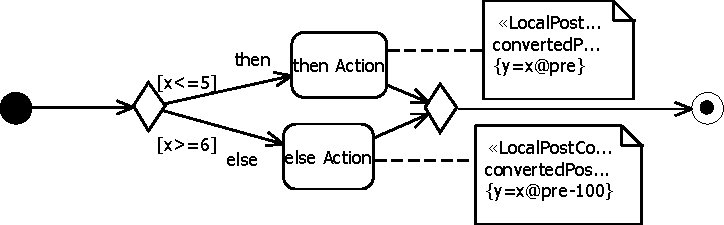
\includegraphics[width=0.7\textwidth]{./pics/BasicExamples.pdf}
\end{center}
\caption{Example of a simple activity with two actions and one decision}
\label{fig:ActivityExample}
\end{figure}
Assume an activity modelling the statement \verb" if (x<=5) then y=x else y=x-100". The corresponding activity diagram is shown in Figure \ref{fig:ActivityExample}. There are two possible control flow paths. Each possible control flow path contains exactly one action. Consequently we need two states: one initial state and one state after the execution of the first action. There are two variables, $x$ and $y$. For each variable we need in AMPL an array of length 2 in order to hold the value assignment for those variables in each state. We will denote the value assignment for $x$ in the i-th state as $x_i$. \\
Let us assume we want to generate test data for the \textsf{{\_}then} path in the diagram. In this case in the initial state the constraint $x_0 \leq 5$ is activated and in the first state we have the constraint $y_1=x_0$ activated. Further, as explained in Section \ref{sec:addingContinuityConstraints}, the continuity constraint $x_0=x_1$ has been introduced automatically since there is no other rule constraining $x_1$ and we want to preserve the variable's value from the previous state when possible. The resulting problem is a linear program with four unknown values and three linear equations and inequalities. The resulting linear program for this case is shown in equations (\ref{eqn:ActivityExample})-(\ref{eqn:ActivityExampleEND}). The linear equations do only represent those constraints that are active for the \textsf{{\_}then} control flow path in the diagram. The constraints $x_0 \geq 6$ and $ y_{1}=x_{0} - 100 $ are not on the \textsf{{\_}then} control flow path. The value of $y_0$ will stay unconstrained, since there is no previous state before the initial state. One can recognise already from this small example that there are quite some $0$ entries in the matrices. For larger problems the matrices tend to become sparse. Many of the solvers we present in the Section \ref{sec:testgenSolvers} will take advantage of sparse matrices when solving the problem.
\begin{eqnarray}
\label{eqn:ActivityExample}
\begin{pmatrix} 1 & 0 & 0 & -1 \\ 1 & -1 & 0 & 0 \end{pmatrix} \times \begin{pmatrix} x_0 \\ x_1 \\ y_0 \\ y_1 \end{pmatrix} = \vec{0} \\
\begin{pmatrix} 1 & 0 & 0 & 0 \end{pmatrix} \times \begin{pmatrix} x_0 \\ x_1 \\ y_0 \\ y_1 \end{pmatrix} \leq \begin{pmatrix} 5 \\ 0 \\ 0 \\ 0 \end{pmatrix}
\label{eqn:ActivityExampleEND}
\end{eqnarray}
%Any variable can be either an integer, a real number or a boolean. Each postcondition, guard condition and invariant will show up as constraint in the AMPL model. In the data to the model we will specify which constraints are activated for which states.  We can also see the set of postconditions as a state transition function. \\
%\subsection{How to Transform an Activity Test Case Graph into a Mathematical Program}
\subsection{Transforming a TCGActivity to an AMPL Model}
\label{sec:atcg2AMPLModel}
Each AMPL model has one parameter called \texttt{pathlength} representing the number of actions on a path. 
For each action with post--conditions and each control flow with a guard there is one \emph{activation set}. An activation set is required to be a subset of $[1..pathlength]$ and specifies those states, in which a post--condition or guard condition is active. 
The value of the parameter \texttt{pathlength} as well as the elements of each activation set will be specified in the AMPL data. In this way there is one AMPL model per activity diagram and any control flow path within the activity diagram can be specified in the AMPL data.\\
The AMPL model built will be synthesised as specified in Algorithm \ref{alg:TCGActivity2AMPL}. We use the `MOF Model--To--Text Transformation' (MOFM2T) language to specify model--to--text transformation. For each variable in the source model there will be one variable declaration, for each action there will be an activation set declared and multiple sets of constraints. For each control flow having a guard condition there will be an activation set and one set of constraints. The synthesis of AMPL code for variables, actions, and guards will be explained in more detail in Section \ref{sec:Variables2AMPL}-\ref{sec:Guards2AMPL} respectively.
\begin{algorithm}
\begin{lstlisting}[numbers=left,escapeinside={@}{@},breaklines=true]
[@\bfseries{template}@ public ActivityToAMPL(act : TCGActivity)]
  param pathlength;
  [@\bfseries{for}@(var : TCGVariable | act.variables)]
    [VariableToAMPL(var)/]
  [/@\bfseries{for}@]
  [@\bfseries{for}@(action : TCGAction | act.nodes)]
    [ActionToAMPL(action)/]
  [/@\bfseries{for}@]
  [@\bfseries{for}@(cf : TCGControlFlow | act.edges)]
    [ControlFlowToAMPL(cf)/]
  [/@\bfseries{for}@]
[/@\bfseries{template}@]
\end{lstlisting}
\caption{Model--to--text transformation from TCGActivity to AMPL model}
\label{alg:TCGActivity2AMPL}
\end{algorithm}
\subsection{Transforming TCGVariables}
\label{sec:Variables2AMPL}
\begin{algorithm}
\begin{lstlisting}[numbers=left,escapeinside={@}{@},breaklines=true]
[@\bfseries{template}@ public VariableToAMPL(var : TCGVariable)]
  var [var.name/] [@\bfseries{if}@ var.isParameter = false] {0..pathlength} [/@\bfseries{if}@] [TypeSpecification(var.type)/] :=1;
[/@\bfseries{template}@]

[@\bfseries{template}@ public Type2AMPL(type : TCGBasicVariableType)]
  [@\bfseries{if}@ type = integer] : integer >=-10000, <= 10000 [/@\bfseries{if}@]
  [@\bfseries{if}@ type = boolean] in 0..1 [/@\bfseries{if}@]
  [@\bfseries{if}@ type = real] >=-10000, <= 10000 [/@\bfseries{if}@]
[/@\bfseries{template}@]
\end{lstlisting}
\caption{Model--to--text transformation from TCGVariable to AMPL model}
\label{alg:TCGVariable2AMPL}
\end{algorithm}
The `MOF Model--To--Text Transformation' (MOFM2T) template to transform a TCGVariable into an AMPL variable declaration is printed in Algorithm \ref{alg:TCGVariable2AMPL}. Every variable has one out of three possible types: integer, real and boolean. In AMPL, by default, a variable is in the domain of real numbers. AMPL also supports variables in the domain of integers. For integers and real numbers we always need an upper and a lower bound that will be set to $+10000$ and $-10000$ by default. Without any bounds at all some solvers can not to produce correct results. The boolean domain is modelled by the set expression $ \left[ 0 .. 1 \right] $, where 0 corresponds to false.\\
Since a variable can have different values in each state of the execution, each variable will be modelled in AMPL as a variable array of fixed size. The size of the array is defined by the \texttt{pathlength}. When the isParameter attribute of the TCGVariable is true then the variable is constant and cannot change its value from one state to another, thus we can model those variables as a single AMPL variable.
\subsection{Transforming LocalPostConditions}
\label{sec:Postconditions2AMPL}
\begin{algorithm}
\begin{lstlisting}[numbers=left,escapeinside={@}{@},breaklines=true]
[@\bfseries{template}@ public ActionToAMPL(action : TCGAction)]
  @\label{lst:activationSet}@set [action.name/] within {0..pathlength} default {};
    [@\bfseries{for}@(constraint : TCGOCLExpression | action.localPostconditions)]
    @\label{lst:constraints}@s.t. [action.name/]_post_[action.localPostconditions->indexOf(constraint)/] {i in action.name} : 
    [ConstraintToAMPL(constraint)/] ;
  [/@\bfseries{for}@]
[/@\bfseries{template}@]

[@\bfseries{template}@ public ConstraintToAMPL(constraint : TCGOCLExpression)]
  [@\bfseries{let}@ func : TCGOCLOperationCallExp]
    @\label{lst:opCall2AMPL}@([ConstraintToAMPL(func.source)/] [func.operation.toOpSymbol()/] [ConstraintToAMPL(func.arguments)/])
  [/@\bfseries{let}@]
  [@\bfseries{let}@ literal : TCGOCLLiteralExp]
    @\label{lst:literal2AMPL}@([literal.value/])
  [/@\bfseries{let}@]
  [@\bfseries{let}@ var : TCGOCLVariableCallExp]
    @\label{lst:varCall}@([var.variable.name/] [@\bfseries{if}@ var.variable.isParameter = false ] [i [@\bfseries{if}@ var.isIsPre] -1 [/@\bfseries{if}@] ] [/@\bfseries{if}@])
  [/@\bfseries{let}@]
[/@\bfseries{template}@]
\end{lstlisting}
\caption{Model--to--text transformation from TCGAction to AMPL model}
\label{alg:TCGAction2AMPL}
\end{algorithm}
For each TCGAction the activation set is declared as a subset of $\left[0..\texttt{pathlength}\right]$ in the AMPL model. The name of the activation set is the name of the TCGAction. The name of each TCGAction is guaranteed to be unique within one activity test case graph model, so name clashes in the AMPL model are prevented (see Section \ref{sec:uml2atcg}). Each local post--condition of an action is transformed into an indexed collection of constraints over the activation set.\\
In Algorithm \ref{alg:TCGAction2AMPL} the transformation of a TCGAction into AMPL code is specified in the MOFM2T language. The ActionToAMPL template first generates the declaration of the activation set, see in line \ref{lst:activationSet}. If no entries are added in the data section it is by default an empty set. In the for--loop the constraint sets are generated for each of the local post--conditions of the current action. In AMPL every constraint needs a name and the name has to be unique. For this reason we are composing the name from the action's name and the index of the current constraint in the ordered list of local post--conditions in line \ref{lst:constraints}.\\
The called \verb=Constraint2AMPL= template (line \ref{lst:constraintsCF}) specifies the actual re--serialisation of the OCL constraint, which was parsed in Section \ref{sec:OCLParsing}, in AMPL syntax. As explained in Section \ref{sec:Variables2AMPL} variables are represented as an array containing one value for each state during the execution. Consequently when a constraint accesses a variable we need to specify in which state that variable is accessed. That is the point where the index from the activation set is used. If the variable reference was marked with \verb�@pre� we are accessing the variable in the previous state and thus need to subtract one from the index; otherwise we access the variable at the index from the activation set. This is shown in line \ref{lst:varCall}. The serialisation of function calls and literals is straightforward as shown in line \ref{lst:opCall2AMPL} and line \ref{lst:literal2AMPL}. The function toOpSymbol() called in line \ref{lst:opCall2AMPL} will generate the appropriate operation symbol representing the TCGOCLOperationType literal it is called on.
\subsection{Transforming Guards}
\label{sec:Guards2AMPL}
\begin{algorithm}
\begin{lstlisting}[numbers=left,escapeinside={@}{@},breaklines=true]
[@\bfseries{template}@ public ControlFlowToAMPL(cf : TCGControlFlow)]
  [@\bfseries{if}@ cf.guard != null /]
    @\label{lst:activationSetCF}@set [cf.name/] within {0..pathlength} default {};
    @\label{lst:constraintsCF}@s.t. [cf.name/]_guard {i in cf.name} : [ConstraintToAMPL(cf.guard)/] ;
  [/@\bfseries{if}@]
[/@\bfseries{template}@]
\end{lstlisting}
\caption{Model--to--text transformation from TCGControlFlow to AMPL model}
\label{alg:TCGControlFlow2AMPL}
\end{algorithm}
The transformation of guards works analogously to the transformation of local post--conditions. The transformation is specified in Algorithm \ref{alg:TCGControlFlow2AMPL}. A control flow can either have a single guard or not. Multiple guards are not possible. If there is no guard no code needs to be produced at all for this control flow. The name of a control flow is guaranteed to be unique within the activity test case graph model to avoid name clashes. In line \ref{lst:activationSetCF} the activation set for the control flow is declared and in line \ref{lst:constraintsCF} the indexed constraint set for the guard is declared. For the actual re-serialisation of the textual OCL in AMPL syntax the ConstraintToAMPL template from Algorithm \ref{alg:TCGAction2AMPL} is used. Guards cannot contain variable references marked with \verb=@pre=, thus the optional decrement of the index in line \ref{lst:varCall} in Algorithm \ref{alg:TCGAction2AMPL} will never be added for a guard.
\subsection{Specifying Control Flow Paths in the AMPL Data}
\label{sec:amplDataGeneration}
\begin{algorithm}
\begin{lstlisting}[language=ampl,numbers=left,escapeinside={@}{@},breaklines=true]
param Pathlength;
var y{0..Pathlength} : integer >=-10000, <= 10000 := 1;
var x{0..Pathlength} : integer >=-10000, <= 10000 := 1;
set else_Action within {0..Pathlength} default {};
s.t. else_Action_post0{i in else_Action} : (y[i])=((x[i-1])-(100.0));
s.t. else_Action_post1{i in else_Action} : (x[i])=(x[i-1]);
set then_Action within {0..Pathlength} default {};
s.t. then_Action_post0{i in then_Action} : (y[i])=(x[i-1]);
s.t. then_Action_post1{i in then_Action} : (x[i])=(x[i-1]);
set _then within {0..Pathlength} default {};
s.t. then_guard{i in then} : (x[i])<=(5.0);
set _else within {0..Pathlength} default {};
s.t. else_guard{i in else} : (x[i])>=(6.0);

DATA
param Pathlength := 1;
set then_Action:= 1;
set then:= 0;
\end{lstlisting}
\caption{Example AMPL model with corresponding data section specifying a control flow path}
\label{alg:ActivityExample}
\end{algorithm}
To clarify how the control flow path will be symbolically executed and encoded in the AMPL data we will refer back to the introductory example shown in Figure \ref{fig:ActivityExample}. The corresponding AMPL model produced by the transformation specified in this chapter we show in Algorithm \ref{alg:ActivityExample}. The last three lines of Algorithm \ref{alg:ActivityExample} contain the \verb=DATA= section. In the \verb=DATA= section we see that the \texttt{pathlength} is 1 and in the first state the constraints of the \textsf{then{\_}Action} are active. In the initial state the constraint of the \textsf{{\_}then} control flow is active. Since there are no cycles in the path every activation set has at most one entry.\\
Keep in mind that the semantics of an activity test case graph is like a Petri--net. In cyclic activity diagrams there are paths that contain one control flow several times. The activation set will then contain one entry for each state in which a token moves along the control flow from the source node to the target node. Actions can be executed several times to move from one state to another, thus the corresponding activation set will then contain the index of the state after execution of the action for each execution.\\
\begin{algorithm}
\begin{algorithmic}[1]
\Require path := ordered set of TCGControlFlows forming a control flow path
\Ensure activationSet contains activation sets representing the given path
\State activationSet(element : AbstractTCGElement) : Integer Set \Comment Mapping from an activity test case graph element to a set of integers. Initially all sets are empty.
\State i $\gets$ 0
\ForAll{cf : TCGControlFlow $\in$ path}
\If{ cf.guard. != null}
\State activationSet(cf).add(i)
\EndIf
\If{ cf.target.oclIsKindOf(TCGAction) }
\State i $\gets$ i+1
\State activationSet(cf.target).add(i)
\EndIf
\EndFor
\end{algorithmic}
\caption{Transformation from a control flow path to a map of activation sets}
\label{alg:controlFlowPathTOActivationSet}
\end{algorithm}
\begin{algorithm}
\begin{lstlisting}[numbers=left,escapeinside={@}{@},breaklines=true]
[@\bfseries{template}@ public ActivationSet2AMPLData{element AbstractTCGElement}/]
[@\bfseries{if}@ ActivationSet(element) != {}/]
set [element.name] :=[@\bfseries{for}@ integer i : ActivationSet(element)] [toString(i)/] [/@\bfseries{for}@] ;
[/@\bfseries{template}@]
\end{lstlisting}
\caption{Text template for printing an activation set in AMPL syntax}
\label{alg:ActivationSetTOAmplDataString}
\end{algorithm}
An algorithm for transforming a control flow path represented as ordered set of control flows into a function mapping every instance of an AbstractTCGElement to an activation set is given in Algorithm \ref{alg:controlFlowPathTOActivationSet}. Every non--empty activation set belonging to an action having local post--conditions or a control flow having a guard needs to be expressed in AMPL syntax; the MOFM2T template for this is shown in Algorithm \ref{alg:ActivationSetTOAmplDataString}.
\section{Abstract Test Case Generation}
\label{sec:pathsearch}
In order to generate a test suite with good model coverage we need to select a set of control flow paths from the activity test case graph that we want to generate test data, and finally create a unit test for. We use a depth first search or alternatively a breadth first search to find suitable control flow paths to generate unit tests from. To ensure that the search is terminating we introduced two parameterised termination conditions. The user can specify the maximum amount of test cases to be found and the maximum length of control flow paths to be tested. There are only finitely many control flow paths up to a certain length within a test case graph. We also specify early infeasible path recognition for the breadth first search. We solve the AMPL program for a control flow path during search and bound the search if the AMPL program was reported to be infeasible.\\
The rest of this section is organized as follows: In Section \ref{sec:pathserachPathTree} we introduce basic concepts and data structures. The algorithms presented in Section \ref{sec:pathsearchBFS} will use those concepts and data structures. The early infeasible path recognition is explained in Section \ref{sec:EarlyInfeasiblePathRecognition}. %Its length is determined by counting the TCGControlFlows in the control flow 
\subsection{Path Tree}
\label{sec:pathserachPathTree}
For the algorithms presented in the following section we need some definitions.
A control flow path is represented as a sequence of control flows. An \emph{abstract test case} is a control flow path starting at the initial node of the activity and ending at a final node. Any node with no outgoing control flow is a final node. For two subsequent control flows, a and b, in a control flow path the OCL expression \texttt{a.target = b.source} is true. \\
We will need the concept of a \emph{path tree} to explain the presented algorithms. We define the \emph{path tree node} as a triple of an edge, the depth, and the predecessor. The edge is a reference to a TCGControlFlow within the examined activity test case graph. The depth is a natural number and predecessor is a reference to another path tree node. The depth of a path tree node is always one more than the depth of its predecessor. A root node does not have a predecessor and its depth is $0$.\\
%A path tree is a tree holding all control flow paths starting at the initial node of an activity. The root \emph{path tree node} is a control flow path of length 0 starting at the initial node of the activity. Each child path tree node of a path tree node p holds a control flow path extending the control flow held by p by one control flow. Thus a path tree node at depth 1 in the path tree is representing a control flow path consisting of one control flow. Every leaf path tree node holds a control flow path from the initial node to a final node of the activity, an abstract test case graph. The path tree for a cyclic activity test case graph is infinite. During the path search we will only construct a partial path tree.\\
%path. A control flow path may contain a single TCGControlFlow multiple times and it will be counted each time.
In the described algorithms the target of a currently examined TCGControlFlow is called \emph{current node}. We call each outgoing edge of the current node a \emph{consequent edge}.\\%Every edge in a control flow path has to be a consequent edge of its predecessor in the control flow path, unless it is the first control flow in the control flow path.
%Bounded BFS, and Bounded DFS, and DFS with early infeasible Path elimination.
%Suggest extending the search algorithms to work with test goals as explained by Stephan Weißleder.
\subsection{Path Search}
We find all abstract test cases in the activity test case graph that have not more than maximum path length control flows. Therefore we construct a path tree from the activity test case graph. The search can be terminated when the maximum amount of test cases is reached. We have two possible orders to construct the path tree: breadth first and depth first.
\begin{algorithm}
\begin{algorithmic}[1]
\Require atcg := A TCGActivity 
\Require MaxDepth := maximum path length of abstract test cases found 
\Require MaxNoPaths := maximum amount of test cases to be found
\Ensure abstractTestCases := set of at most MaxNoPaths abstract test cases consisting of at most MaxDepth TCGControlFlows each
\State abstractTestCases $\gets$ initially empty set of control flow paths \Comment initialisation
%\State currentPath $\gets$ initially empty control flow path
\State queue $\gets$ initially empty queue of path tree nodes
\For {edge : TCGControlFlow $\in$ atcg.initialNode.outgoing}
 \State queu.put((edge, 0, null))  \Comment Add root path tree nodes
\EndFor \Comment end initialisation
\While{queue is not empty \textbf{and} abstractTestCases->size() $\leq$ MaxNoPaths}
 \State ptNode $\gets$ queue.get() \Comment visit next search tree node from the queue
 \If{ptNode.depth $\leq$ MaxDepth} \label{line:BFSifFeasible}
  \For{edge : TCGControlFlow $\in$ currentEdge.edge.target.outgoing}
   \State queue.put((edge,ptNode.depth,ptNode))\Comment Add successor nodes to queue
  \EndFor
 \EndIf
 \If{currentEdge.edge.target.outgoing->size()=0} \Comment final node found
  \State path $\gets$ reconstruct control flow path from the edge in the root path tree node to ptNode.edge by traversing predecessors
  \State abstractTestCases.add(path) \Comment 
 \EndIf
\EndWhile
\end{algorithmic}
\caption{Breadth first search algorithm to generate abstract test cases from an activity test case graph}
\label{alg:BreadthFirstSearch}
\end{algorithm}
\subsubsection{Breadth First Search}
\label{sec:pathsearchBFS}
% \begin{algorithm}
% \begin{algorithmic}
% \Require atcg := A TCGActivity \\
% MaxDepth := maximum path length for each control flow path \\
% MaxNoPaths := maximum amount of different control flow paths to be found
% \Ensure abstractTestCases := set of at most MaxNoPaths control flow paths consisting of at most MaxDepth TCGControlFlows each\\
% \State abstractTestCases $\gets$ initially empty set of control flow paths \Comment initialisation
% \State queue $\gets$ initially empty queue of path tree nodes
% \For {TCGControlFlow edge $\in$ atcg.initialNode->outgoing}
% \State queue.put((edge, 0, null)) \Comment Add root path tree nodes
% \EndFor \Comment end initialisation
% 
% \While{queue is not empty \textbf {and} abstractTestCases.size $\leq$ MaxNoPaths}
% \State ptNode $\gets$ queue.get() \Comment visit next path tree node from the queue
% \If{ptNode.depth $\leq$ MaxDepth} \label{line:BFSifFeasible}\Comment search only up to MaxDepth
% \For{TCGControlFlow edge $\in$ ptNode.first.target->outgoing}
% \State queue.put((edge, ptNode.depth + 1, ptNode)) \Comment Add successor nodes to queue
% \EndFor
% \EndIf
% \If{ptNode.first.target->outgoing.size()=0} \Comment A final node has been found
% \State path $\gets$ reconstruct control flow path from the edge in the root path tree node to ptNode.edge by traversing predecessors
% \State abstractTestCases.add(path) \Comment 
% \EndIf
% \EndWhile
% \end{algorithmic}
% \caption{Breadth first search algorithm to generate control flow paths from an activity test case graph}
% \label{alg:BreadthFirstSearch}
% \end{algorithm}
%In the basic depth first search one will visit each node but cannot reconstruct the path taken to this node. Our goal is to find all paths so we need a data structure that enables us to reconstruct the path up to the current node. Throughout the search we are building a \emph{path tree}. We define the path tree node as a triple of an edge, the depth, and the predecessor. The edge is a reference to a TCGControlFlow within the examined activity test case graph. The depth is a natural number and predecessor is a reference to another path tree node. The depth of a path tree node is always one more than the depth of its predecessor. A root node does not have a predecessor and its depth is $0$.\\
In breadth first search we find all control flow paths of length $n$ before a control flow path of length $n+1$ is examined. 
We use a queue to store path tree nodes and examine them in first--in--first--out order. Algorithm \ref{alg:BreadthFirstSearch} shows the pseudo code of the algorithm based on breadth first search. We initially start by generating root path tree nodes for each outgoing edge of the initial node. In each round one path tree node is retrieved from the queue. We add a new path tree node to the queue for each consequent edge if the current depth is smaller than the maximum path length (MaxDepth). When a final node with no more outgoing edges has been found, we can traverse the path of predecessors back to the root path tree node and construct an abstract test case. The algorithm will halt when either all paths up to MaxDepth length have been found or the number of paths found exceeds the maximum amount of test cases (MaxNoPaths).
\subsubsection{Depth First Search}
\label{sec:pathsearchDFS}
During the depth first search, we will always find the abstract test case next that has the longest common sub--path with the last found abstract test case. It works exactly like the breadth first search, just replace the first--in--first--out queue with a last--in--first--out stack in Algorithm \ref{alg:BreadthFirstSearch}. For the implementation this algorithm can be more efficient since it is not necessary to keep the complete path tree until the search is done. As soon as all successors of a path tree node have been found, the path tree node can be discarded.
% %incrementally build a control flow path and use a stack to remember all the path tree nodes that we have not yet examined. Algorithm \ref{alg:DepthFirstSearch} shows our depth first search based algorithm generating abstract test cases. % In a cyclic graph it makes a difference whether we are traversing edge after 2 iterations of a cycle or after 3 iterations of a cycle. This fact makes it necessary to store the length of the sub--path up to the edge along with the edge to be examined in the stack.
% Initially we push one path tree node for each outgoing edge of the initial node together with the depth $0$. We do not need to remember predecessors for this algorithm. In each step we pop the next path tree node from the stack and in a simple forward step it will be the path tree node we just pushed and the edge can be appended to the current path. Then we create one path tree node containing each following edge and the current depth. If in the last step a final node has been found or the maximum depth has been reached there will be no subsequent edge on the stack but we will have to backtrack. During backtracking we remove the last edges from the current path until the path has the path length given by the depth of the path tree node just popped from the stack. 
\subsection{Early Infeasible Path Elimination}
\label{sec:EarlyInfeasiblePathRecognition}
When searching for abstract test cases as shown in the subsections before, it may happen that the constraints along a control flow path found are unsatisfiable. That means there is no valid input data that will cause the execution of this path. Let us, for example, consider a control flow path containing one TCGControlFlow with the guard $x\leq 5$ and another TCGControlFlow with the guard $x\geq 10$, and in between those two control flows there is no TCGAction changing the value of $x$. Obviously, there is no possible value for $x$ fulfilling those two constraints. When no valid input data for a certain control flow path can be found we call that control flow path an \emph{infeasible path}.\\
\subsubsection{Advantages of Early Infeasible Path Recognition}
The most important advantage of infeasible path recognition is that we can bound the search for abstract test cases. If a control flow path is infeasible then no extension of that control flow path will be feasible. The number of control flow paths found may grow exponentially with the maximum path length. If we assume a large graph where, in average, each node has two outgoing edges we will get 1024 paths of length 10. When one control flow path of length 3 was already infeasible then there are 128 infeasible paths of length 10. We can avoid many fruitless searches by excluding infeasible paths as early as possible.\\
When the abstract test case generating algorithm is capable of infeasible path recognition the user can also control that the set of abstract test cases found is finite by adding additional control flows before each loop in the activity diagram. The guard of the additionally added control flow must contain a constraint on the loop variant. Thus most control flow paths containing arbitrary many iterations of this loop will be excluded from the abstract test case generation. For example, when we model a simple counter loop decreasing some counter variable $i$ to 0 we can specify in the guard before the loop that the counter variable may be between 3 and 5. In this case the path search algorithm with infeasible path recognition will find only those paths where the loop is iterated between three and five times.\\
Furthermore, it is useless to generate abstract test cases that are infeasible since infeasible abstract test cases can not be transformed into test cases.
\subsubsection{The Algorithm}
When using the breadth first or the depth first search approach we can generate abstract test cases and pass them on to the next step in the unit test generation algorithm, where infeasible paths will be detected. When we want to check whether a currently examined control flow sub path is a feasible path we will interleave the \nameref{sec:pathsearch} step with the \nameref{sec:testgenerationSolving} step.\\
Only a slight modification of Algorithm \ref{alg:BreadthFirstSearch} is necessary to enable early infeasible path elimination for our breadth first search based algorithm: the condition in line \ref{line:BFSifFeasible} needs to be extended. It controls whether a path tree node will be added for the consequent edges or not. We additionally need to check whether the control flow path, which is represented by the current path tree node (ptNode), is feasible. The check for feasibility is done by generating the AMPL data for the control flow path represented by the current path tree node and solving the problem as explained in Section \ref{sec:testgenCallingtheSolver}. The generation of the AMPL data from a control flow path was explained in Section \ref{sec:amplDataGeneration}. For infeasible path detection we will analyse the indication returned from the solver. If the solver reports `solved', `solved?', or `unbound' the examined control flow path is feasible. If the solver reports `infeasible' or `failure' we assume the examined control flow path to be infeasible.
\section{Specific Test Data Generation}
\label{sec:testgenerationSolving}
For every abstract test case found during \nameref{sec:pathsearch} we want to generate a test case. A test case contains input values for every parameter of the function under test, initial values for fields, and the corresponding expected output values. Test cases are stored in a unit test model. From a unit test model we can easily generate unit tests for any programming language. In Section \ref{sec:testgenerationUnitTestSynthesis} we will present a MOFM2T template that generates C++ unit tests from a unit test model. The unit test meta model is explained in Section \ref{sec:testMetaModel}. \\
In order to get numerical values for the parameters and fields of the unit under test we have a constraint satisfaction problem solved for each abstract test case. The constraint satisfaction problem to solve for each abstract test case is encoded as AMPL program according to the specification given in Section \ref{sec:atcg2Ampl}. The AMPL program will be solved by one of the solvers interfacing the AMPL system. An overview of the solvers we tried out for this thesis is given in Section \ref{sec:testgenSolvers}. How we interact with the AMPL system, is explained in more detail in Section \ref{sec:testgenCallingtheSolver}.
When testing, often errors are triggered by test data that is exactly on the boundary of one or more decisions. For example, when we test the decision \texttt{if x<=5 then\ldots} the test value $x=5$ will cause the test to fail when the $\leq$ has been replaced by a $<$; other test values will not trigger this fault. How we can ensure to find such boundary values, is explained in Section \ref{sec:boundaryValueSelection}.\\
The AMPL encoding ensures that we can use the same AMPL model for every control flow path within one activity. Each control flow path and any sub--path within an activity can be specified via the AMPL data, which is not part of the AMPL model and can be modified interactively. The fact that we use the same model for several solver invocations in a row enables us to use the warm start capabilities of many solvers to speed up the computation, as we will show in Section \ref{sec:AMPLWarmStartCapabilities}.\\
%In the constraint satisfaction problem we solve the values at the boundary of the feasible set are corresponding to the values at the boundary of decisions in the control flow. We can use some background knowledge about the algorithms to steer properties of the obtained test data, especially whether the obtained solution is on the boundary of the feasible set or somewhere in the middle.
%Sch�n gemacht!
\subsection{The Unit Test Meta Model}
\label{sec:testMetaModel}
\begin{figure}
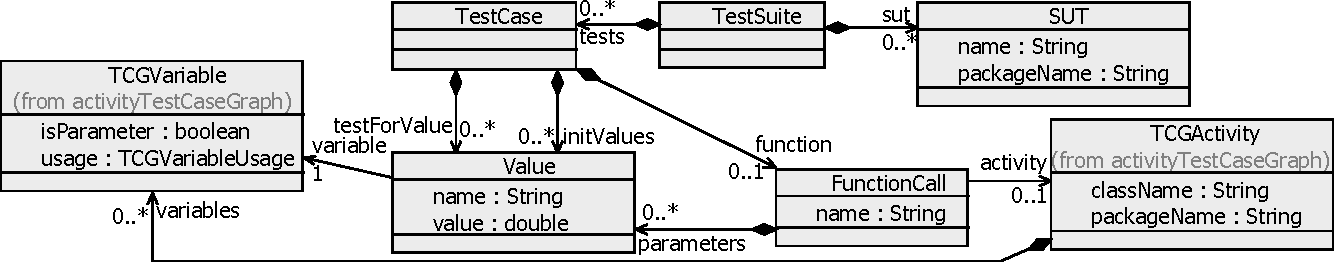
\includegraphics[width=\textwidth]{./pics/Tests.pdf}
\caption{The unit test meta model}
\label{fig:UnitTestMetaModel}
\end{figure}
The unit test model serves as interface between the \nameref{sec:testgenerationSolving} and the \nameref{sec:testgenerationUnitTestSynthesis}. All information needed to build a compilable unit test for the function that is modelled by the activity is contained in a unit test model. The unit test model is completely independent from the programming language and the unit test framework used for testing.\\%Thanks to the model representation of unit tests the \nameref{sec:Normalisation}, \nameref{sec:atcg2Ampl}, \nameref{sec:pathsearch}, and the \nameref{sec:testgenerationSolving} 
In Figure \ref{fig:UnitTestMetaModel} we depict the meta model of the unit test model. The root element of a unit test model is a TestSuite. A TestSuite can contain several TestCases. Each TestCase consists of two sets of Values and a FunctionCall. The Values in the initValues reference are meant to be used for initialisation of fields. The Values referenced by the testForValue reference specify which value the corresponding fields need to hold after the tested function has been executed. If any field in the system under test does not hold the specified value the test case has failed. The FunctionCall held by the function reference has a name and a reference to the activity test case graph specifying the behaviour of the function under test. The FunctionCall also contains Values in the parameters reference. The Values referenced by the parameter's reference of the FunctionCall specify the input arguments to pass to the function under test when calling it.
\subsection{Solving a Constraint Satisfaction Problem with AMPL}
\label{sec:testgenCallingtheSolver}
For each abstract test case a constraint satisfaction problem needs to be solved in order to obtain numerical values that can be used as test data in a unit test. The constraint satisfaction problem is encoded in AMPL and consists of the AMPL model that is constant for an activity test case graph and the AMPL data that is generated for each abstract test case.\\
The solving of constraint satisfaction problems is done by a solver hooked to AMPL. We start an AMPL instance in a separate process and communicate with this process through its standard input and output streams. First, we load the AMPL model corresponding to the activity test case graph into the AMPL console. We will also ask the user which solver to use for all control flow paths within this model and set AMPL's solver options accordingly through the AMPL console. Then we produce test data for each abstract test case. \\
To produce test data for one abstract test case or control flow path we reset the data currently loaded in AMPL, encode the control flow path as AMPL data according to the specification in Section \ref{sec:amplDataGeneration}, and load the new data in the AMPL console. Now we have AMPL invoke the selected solver. Depending on the solver and the problem the loaded constraint satisfaction problem is an instance of, the computation time varies and we can get one of five possible indications from the solver:
%For each activity test case graph we start one external AMPL process and load the corresponding AMPL model. 
\begin{description}
\item[solved] The solver was able to compute a valid solution to the problem.
\item[solved?] The solver heuristically computed an answer but can not prove that it is correct or optimal.
\item[infeasible] There is no valid input data for the given control flow path or the used heuristics was not lucky.
\item[unbound] The given objective function has no upper bound.
\item[failure] There has been an error condition in the solver routine, for example, division by zero.
\end{description}
If the solver indicates `solved' or `solved?' we will use the values stored in the AMPL variables to produce test cases (Section \ref{sec:AMPLstoringUnitTestModel}). For all other indications we can not produce a test case from the computed data.
\subsection{Storing the Variable Values in a Unit Test Case Model}
\label{sec:AMPLstoringUnitTestModel}
\begin{algorithm}
\begin{algorithmic}[1]
\Require testsuite := A TestSuite element used as root element to contain the produced test cases
\Require A solver has successfully solved a constraint satisfaction problem
\Ensure testsuite contains a TestCase for the last successfully solved abstract test case
\State testCase $\gets$ a new TestCase instance
\State functionCall $\gets$ a new FunctionCall instance
\State testCase.function $\gets$ functionCall
\For {tcgvar : TCGBasicVariable $\in$ tcgActivity->variables}
\If {tcgvar.isParameter = false}
\State v $\gets$ createValue(tcgvar)
\State v.value $\gets$ AMPL(tcgvar.name)$[0]$
\State testCase.initValues.add(v)
\State v $\gets$ createValue(tcgvar)
\State v.value $\gets$ AMPL(tcgvar.name)$[last]$
\State testCase.testForValue.add(v)
\Else
\State v $\gets$ createValue(tcgvar)
\State v.value $\gets$ AMPL(tcgvar.name)
\If {tcgvar.usage = in parameter}
\State functionCall.parameters.add(v)
\EndIf
\If {tcgvar.usage = out parameter \textbf{or} tcgvar.usage = return parameter}
\State testCase.testForValue.add(v)
\EndIf
\EndIf
\EndFor
\end{algorithmic}
\caption{Algorithm transforming a solution of a CSP into a TestCase}
\label{alg:TestCaseModelGen}
\end{algorithm}
When a solver successfully computed an answer for a given constraint satisfaction problem we read the assigned values and store them in a test case model. In Algorithm \ref{alg:TestCaseModelGen} we see the pseudo code of the algorithm creating a TestCase object from the values computed by the constraint solver. We assume that the function AMPL(`x') returns the content of the AMPL variable or variable array x as array. The function createValue(var : TCGVariable) creates a new Value object with its name attribute set to var.name and its variable reference pointing to var.\\
The root element of a test case model is a TestSuite. We will create one TestSuite element for a TCGActivity. For each abstract test case on that TCGActivity that has been successfully solved we will create one TestCase and add it to the TestSuite. For each TCGVariable with its isParameter attribute set to false in the TCGActivity we will retrieve an array of values from the AMPL process. The first value in this array is stored in a Value element. The name of this Value element is set to the name of the TCGVariable and it is added to the initValues reference of the TestCase. In the same way, the last element from the array retrieved from AMPL will be stored in a Value element and stored in the testForValue reference. A FunctionCall with the same name as the TCGActivity will be created. For each TCGVariable with its isParameter attribute set to true a single value will be retrieved from AMPL, and, depending on the usage property of the TCGVariable, the produced Value element will be stored either in the FunctionCall�s parameters or the TestCase�s testForValue reference. For out parameters and return parameters the Value elements are stored in the testForValue set. For in parameters the Value element is stored in the FunctionCall�s parameters.
\subsection{Review of Available Solvers}
\label{sec:testgenSolvers}
A central point of our approach for unit test generation is the application of state--of--the--art constraint solvers to the constraint satisfaction problem that we have generated from a UML activity diagram. As we have explained in Section \ref{sec:Maths} there are several specializations of the constraint satisfaction problem for which algorithms or heuristics exist. Every available solver implements one or more algorithms or heuristics. Thus a solver is suitable for instances of one or more of the presented problems. Table \ref{tab:solvers} contains in each row the name of the solver and a check mark for each problem we have successfully tested it for. 
\begin{table}\begin{center}
\begin{tabular}{l r r r r r r r r}
Solver & LP & MILP & COP & OP & SAT & SMT & FCSP & MINLP\\
\hline
Cplex & \checkmark & \checkmark & & & & & &\\
IlogCP\cite{ilogcp} & \checkmark & \checkmark & & & \checkmark & \checkmark & \checkmark &\\
GeCoDE\cite{gecode} & & & & &\checkmark & \checkmark & \checkmark &\\
JaCoP & & & & &\checkmark & & \checkmark &\\
Couenne\cite{Belotti09couenne} & \checkmark & \checkmark & \checkmark & \checkmark & & & & \checkmark\\
Gurobi & \checkmark & & \checkmark & & & & &\\
LPsolve\cite{lpsolve} & \checkmark &\checkmark  & & & & & &\\
Minos &\checkmark & &\checkmark & & & & &\\
% conopt & & & & & & & &\\
% knitro & & & & & & & &\\
% snopt & & & & & & & &\\
% xpress & & & & & & & &\\
% bonmin & & & & & & & &\\
% cbc & & & & & & & &\\
% ipopt & & & & & & & &\\
\hline
\end{tabular}
\end{center}
\caption{List of solvers and problems they can solve.}
\label{tab:solvers}
\end{table}
\subsection{Warm Start Capabilities} 
\label{sec:AMPLWarmStartCapabilities}
To speed up the computation we use the warm start capabilities of AMPL and most of its solvers. A warm start means that we are solving the same constraint satisfaction problem multiple times in a row but each time with different data. In subsequent runs the solver can reuse knowledge it has gained throughout previous runs and thus generate solutions faster. Using the warm start capabilities requires all problems being solved in the same process and keeping the AMPL model constant. Keeping the AMPL model constant is achieved by the transformation of a TCGActivity to an AMPL model, which allows specifying control flow paths in the data.\\
\begin{figure}
\begin{center}
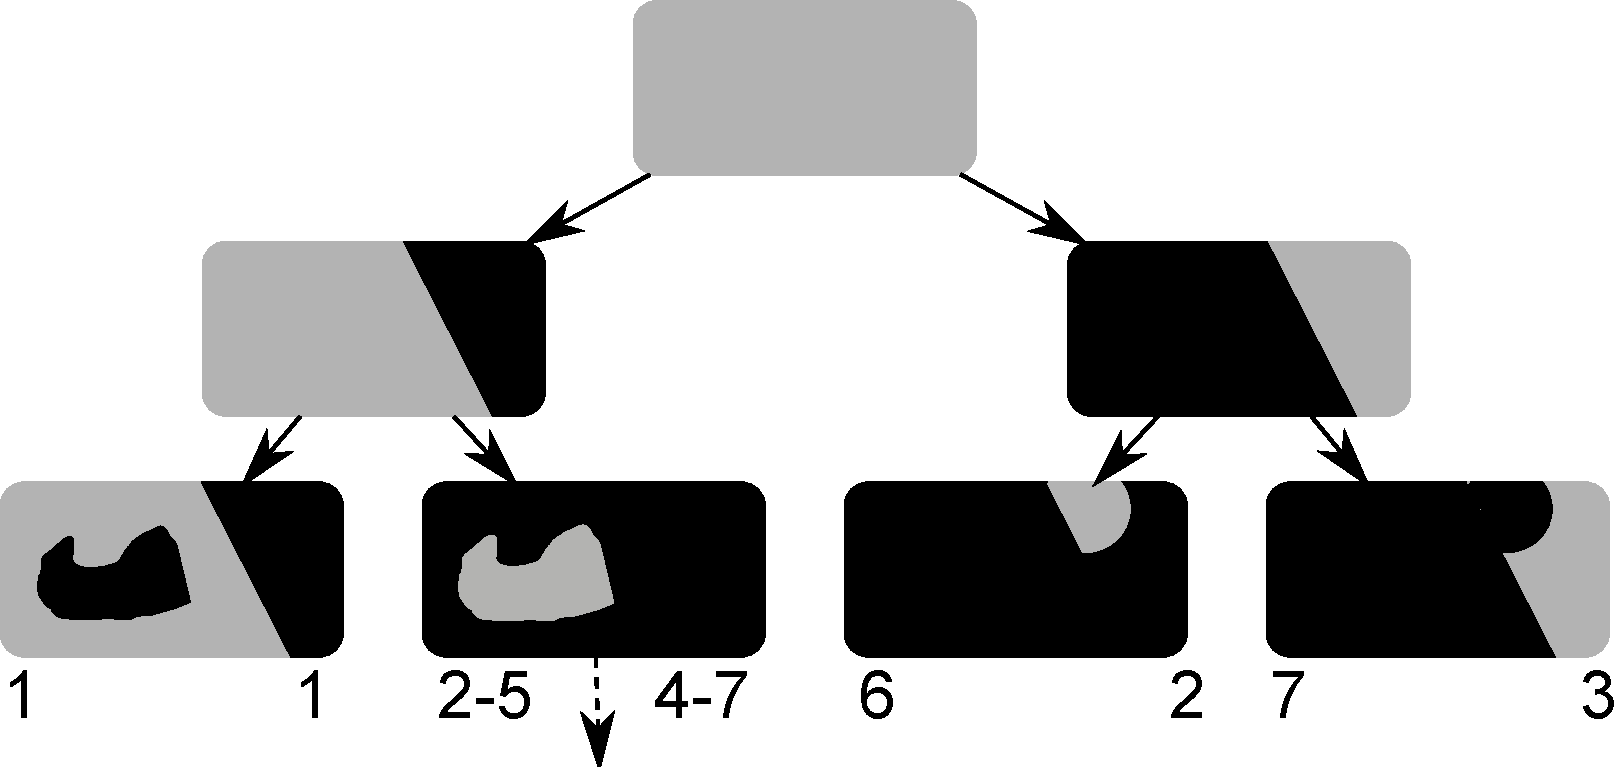
\includegraphics[width=0.6\textwidth]{./pics/VennTree.pdf}
\end{center}
\caption{Venn diagrams for different paths and their ordering}
\label{fig:VennTree}
\end{figure}
Even if the solver is changed between two runs or the solver does not build internal knowledge about the given problem AMPL will store the last answer computed. Many algorithms need a starting point and they will use the last answer computed. In Figure \ref{fig:VennTree} we show a path tree. Each leaf node represents an abstract test case; each intermediate node represents a sub--path from the initial node to some node in the activity test case graph. At each node in the path tree there is a Venn diagram visualising the feasible set of input data for that sub--path. Adding a constraint will never increase the feasible set. Consequently, the feasible set of a path extending another path will always be smaller than the feasible set of its predecessor. The feasible set of a sub--path will always be exactly the union of the feasible set of its successors and the intersection of feasible sets of siblings in the path tree will always be empty. If that were not the case there would be input data for which the control flow is unspecified or non--deterministic. The number on the left of each leaf node gives the order in which the leaf nodes are found by a depth first search and the number on the right of each leaf node gives the order in which they are found by a breadth first search.\\ 
Usually, it is easier to solve a constraint satisfaction problem if we know a starting point that fulfils all constraints except one instead of a starting point violating the majority of the constraints. If we have a solution for a sub--path it is already a feasible solution for one of its successors. If we have a solution for a leaf node we can easily obtain the solution for one of its siblings. Siblings in the path tree share all but one guard condition that means there is only one condition violated if we use the solution from a sibling as starting point. For optimisation problems we have a high chance to move into the feasible region of its sibling by applying a simple local steepest descent search on the objective function augmented by quadratic penalty terms. In the order produced by depth first search, abstract test cases sharing a long common sub--path are next to each other and will, consequently, be solved right after each other. In breadth first order we can see that the fourth abstract test case will use a starting point not fulfilling any constraint for this path. Especially when we solve the constraint satisfaction problems for the intermediate nodes in the path tree - as it is done for the early infeasible path recognition explained in Section \ref{sec:EarlyInfeasiblePathRecognition} - we should memorise the solutions found and set the starting points accordingly before we solve the constraint satisfaction problem for a subsequent path tree node.
\subsection{Boundary Value Analysis}
\label{sec:boundaryValueSelection}
As already motivated, a solution at the boundary of the feasible set for a certain abstract test case is more valuable than other solutions within the feasible set. For linear problems the simplex algorithm will automatically generate only boundary values since it is the nature of the simplex algorithm to move along the exposed points of a polyeder. For all other methods and generating a specific boundary value is a bit more complicated.\\
So far the solved constraint satisfaction problems do not contain an optimisation constraint. Thus, all algorithms terminate as soon as they found any feasible point. In AMPL we can interactively add an objective function before launching the solver for a certain problem. We add an objective function in a way that the optimal point is somewhere at the boundary of the feasible set. Any linear objective function will serve this purpose. After the addition of a linear objective function three things can happen: either the solver returns a boundary value in the next run, or the solver reports that the problem is unbounded, or the solving time for the problem suddenly increases enormously. In the first case everything went fine. If the feasible region is a convex set not containing infinity this will always be the case. The second case indicates that the direction of the objective function points into a direction, where the feasible set is open. In this case we can change the direction of the objective function and try again to hit a boundary. The last case is especially a problem of mixed integer non--linear programs and optimisation problems. It is not too hard to find a feasible solution for one of these problems, when there are enough solutions. Finding an optimal solution for a mixed integer or non--linear program is much harder. We actually don't require a global optimum; a local optimum is at the boundary of the feasible region as well. %In the worst case we need to find all feasible or locally optimal solutions and compare all of them with each other. 
In such a case we can first solve the problem without objective, and when a feasible starting point is available, we apply a local search on the problem with objective and we will not necessarily obtain the global maximum but a local maximum that is at the boundary of the feasible set. We suggest using the last explained procedure to find as many boundary values for each abstract test case as the user demands. The used objective functions may also be provided by the user. We have successfully tested this procedure for mixed integer non--linear programs with the solvers Couenne to find a feasible point and Minos to perform the local search (Section \ref{sec:exampleModelNonConvex}). In Section \ref{sec:caseStudyBoundaryValues} we will also demonstrate in our case study that generating test data at a specific boundary of the feasible region does not increase the overall runtime of our algorithm at all.
\section{Unit Test Synthesis}
\label{sec:testgenerationUnitTestSynthesis}
\begin{algorithm}
\begin{lstlisting}[numbers=left,escapeinside={@}{@},breaklines=true]
[@\bfseries{template}@ public UnitTestToBoostUnitTest(ts : TestSuite) { int count = -1; TCGVariable return = ""; }]
  #define BOOST_TEST_MAIN MyTest
  #include <boost/test/included/unit_test.hpp>
  [@\bfseries{for}@(sut : SUT | ts.sut)]
    #include [sut.packageName/]/[sut.name/].h
  [/@\bfseries{for}@]
  [@\bfseries{for}@(tc : TestCase | ts.tests) { count = count + 1; TCGVariable ret = tc.function.activity.variables->select(v : v.usage = return parameter)}]
    BOOST_AUTO_TEST_CASE( test[count/] ){@\label{line:forEachTestCase}@
    //field initialisation
    [@\bfseries{for}@( v : Value | tc.initValues)]
      [v.name/] = [v.value/];
    [/@\bfseries{for}@]
    //input parameter declaration
    [@\bfseries{for}@( v : Value | tc.function.parameters)]
      const [v.type/] [v.name/] = [v.value/];
    [/@\bfseries{for}@]
    //output parameter declarations
    [@\bfseries{for}@( var : TCGVariable | tc.function.activity.variables->select( var : TCGVariable | var.usage = out parameter))]
      [var.type/] [var.name/]; 
    [/@\bfseries{for}@]
    [ret.type/] [ret.name/];
    //call function under test @\label{line:callFuncUnderTest}@
    [ret.name/] = [tc.function.name/]( [@\bfseries{for}@( var : TCGVariable | tc.function.activity.variables->select( v : TCGVariable | v.isParameter = true and not v.usage = return parameter)) separator(',')] &[var.name/] [/@\bfseries{for}@]) @\label{line:callFuncUnderTestEnd}@
    //check fields, return parameter and output parameters for correct values
    [@\bfseries{for}@( v : Value | tc.testForValue)]
      [@\bfseries{if}@(v.variable.variableType=boolean or v.variable.variableType = integer)] 
        BOOST_CHECK_EQUAL([v.name/],[v.value/]);
      [/@\bfseries{if}@]
      [@\bfseries{if}@(v.variable.variableType=real)] 
        BOOST_WARN_EQUAL([v.name/],[v.value/]);@\label{line:BoostWarn}@
        BOOST_CHECK_CLOSE([v.name/],[v.value/], 0.001);
      [/@\bfseries{if}@]
    [/@\bfseries{for}@]
    }@\label{line:forEachTestCaseEnd}@
  [/@\bfseries{for}@]
[/@\bfseries{template}@]
\end{lstlisting}
\caption{MOFM2T template of a C++ unit test using Boost test library}
\label{alg:boostTemplate}
\end{algorithm}
From a unit test model and the corresponding activity test case graph model we are able to write compilable unit test in any language, using any unit test framework we want. In this Section we will explain an example MOFM2T template (Algorithm \ref{alg:boostTemplate}) that generates C++ unit tests suitable to test C functions. We use the Boost test library as unit test framework. \\
First, we need to include the Boost header and the headers for the system under test. For each TestCase in the TestSuite we print one test case. What is printed for each TestCase can be found in the lines \ref{line:forEachTestCase}--\ref{line:forEachTestCaseEnd}. The central element of each test case is a call to the function under test (lines \ref{line:callFuncUnderTest}--\ref{line:callFuncUnderTestEnd}). Every time data is needed either for initialisation or to verify the results of the function call we will use a value stored inside a Value element of the unit test model. Before the function call we initialise the fields of the system under test and create local variables to pass as input arguments into the function. We also declare uninitialised local variables to receive the output parameters and the return value from the function call. After the function call every variable holding a value that needs to be checked will be checked. For variables in a discrete domain we check for equalities and for floating point variables we check for similarity. Thus a test will not fail due to a small rounding error, but we will generate a warning if a small rounding error occurred (line \ref{line:BoostWarn}). 
% \section{Implementation}
% \label{sec:testgenerationImplementation}
% say a few words about EMF and Eclipse plug--in. Tell that I used Eclipse org.eclipse.ocl.uml and eclipse org.eclipse.uml2.uml packages. 
% \subsection{The Eclipse Modelling Framework}
% \cite{EMF}
% \subsubsection{Importing Models from Atego Artisan Studio}
% \subsubsection{Model transformations}
% \subsubsection{Parsing OCL Expressions}
% \subsection{Using the Resulting Plug--in}
% 


